\subsection{\labeltext[Diagrama de Atividades - Administrador]{Diagrama de Atividades - Administrador}{er:242}}

\begin{figure}[H]
	\centering
	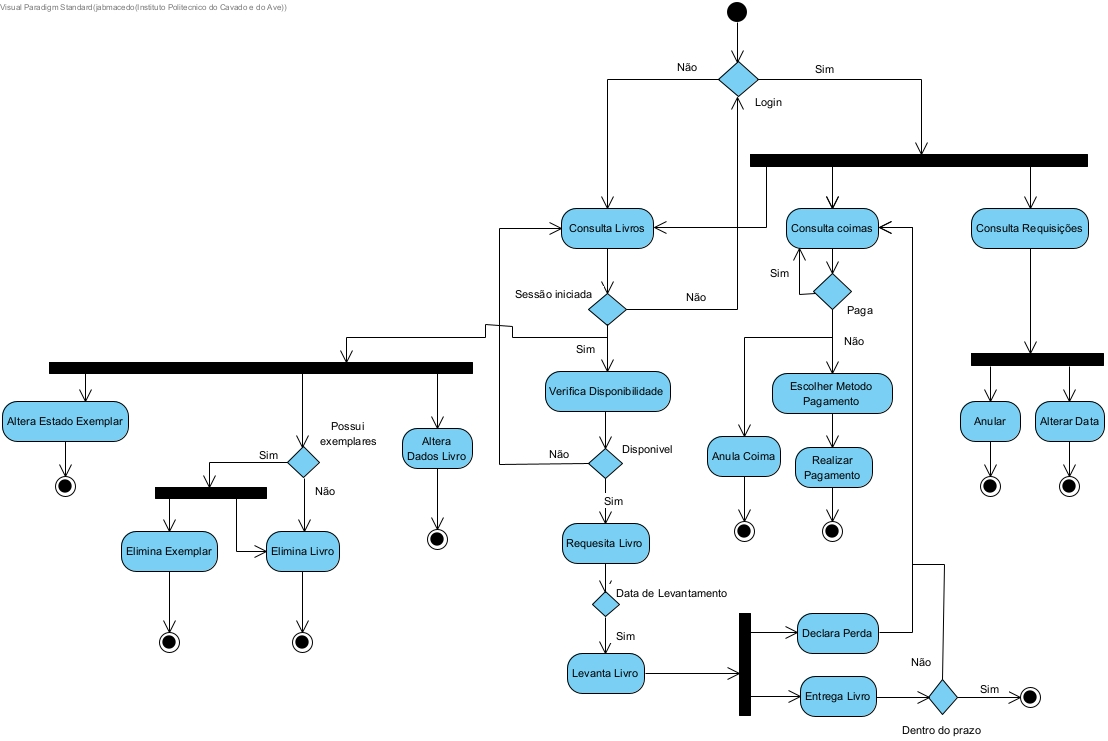
\includegraphics[width=1\linewidth]{./img/Diagramas_A/DA_Admin.jpg}  % largura percentual 
	\caption{\ref{er:242}}
	\label{fig:chap242}
\end{figure}

Como era de esperar, o administrador da biblioteca, ou qualquer user com o tipo admin, ter acesso ao maior numero de funcionalidades e maior liberdade de manipulação de dados.
O Admin pode realizar a eliminação de exemplares e livros, alterações manuais aos seus estados, assim como anular coimas, anular/alterar requisições, entre outras.
A maioria das funcionalidades são identicas para todos os utilizadores como o registo de uma requisição, a forma como as mesmas são geridas, consulta dos livros, consulta das coimas e a gestão das mesmas, sendo apenas aplicadas determinadas regras de negócio que permitem a existencia de uma hierarquia de ações que podem, se mal geridas, corromper todo o sistema.